\documentclass[a4paper]{article}
%\usepackage[utf8]{inputenc}
\usepackage[spanish, es-tabla, es-noshorthands]{babel}
\usepackage[table,xcdraw,dvipsnames]{xcolor}
\usepackage[a4paper, footnotesep=1.25cm, headheight=1.25cm, top=2.54cm, left=2.54cm,
 bottom=2.54cm, right=2.54cm]{geometry}
%\geometry{showframe}
 \usepackage[normalem]{ulem}
 \useunder{\uline}{\ul}{}

%VERIFICAR EL HEAD Y EL FOOT EN
%https://ctan.dcc.uchile.cl/macros/latex/contrib/geometry/geometry.pdf

%Paquetes varios:
\usepackage{verbatimbox}

%\usepackage{wrapfig}			%Wrap figure in text
\usepackage[export]{adjustbox}	%Move images
\usepackage{changepage}			%Move tables
\usepackage{todonotes}

\usepackage{tikz}
\usepackage{amsmath}
\usepackage{amsfonts}
\usepackage{amssymb}
\usepackage{float}
\usepackage[graphicx]{realboxes}
\usepackage{caption}
\usepackage{subcaption}
\usepackage{multicol}
\usepackage{multirow}
\setlength{\doublerulesep}{\arrayrulewidth}
%\usepackage{booktabs}

\usepackage{array}
\newcolumntype{C}[1]{>{\centering\let\newline\\\arraybackslash\hspace{0pt}}m{#1}}
%\usepackage[american]{circuitikz}
\usetikzlibrary{calc}
\usepackage{fancyhdr}
\usepackage{units} 

\usepackage{colortbl}
%\usepackage{sectsty}
%\usepackage{unicode-math}

%FONTS (IMPORTANTE): Compilar en XeLaTex o LuaLaTeX
\usepackage{anyfontsize}	%Font size
\usepackage{fontspec}		%Font type
%Si sigue sin andar comentar \usepackage[utf8]{inputenc}
%https://ctan.dcc.uchile.cl/macros/unicodetex/latex/fontspec/fontspec.pdf
%https://www.overleaf.com/learn/latex/XeLaTeX

%Path para imagenes para trabajar en subarchivos
\graphicspath{{../Resumen/}{../Referencias/}{../Apendice/}{../Descripción de la Empresa/}{../Tareas del Alumno/}{../Conclusiones/}{../Herramientas Empleadas/}}

%Definiciones de nuevos comandos y colores
%COLORES:
\definecolor{AzulFoot}{rgb}{0.682,0.809,0.926}	%RGB	%{174,206,235}
\definecolor{AzulInfo}{rgb}{0.180,0.455,0.710}	%RGB	%{46,116,181}
\definecolor{AzulTable}{rgb}{0.302,0.507,0.871}	%RGB	%{68,114,196}
\definecolor{PName}{rgb}{0.353,0.353,0.353}		%RGB	%{90,90,90}
\definecolor{mygreen}{rgb}{28,172,0} % color values Red, Green, Blue
\definecolor{mylilas}{rgb}{170,55,241}

%Change Font Size

% #1 = size, #2 = text
\newcommand{\setparagraphsize}[2]{{\fontsize{#1}{6}\selectfont#2 \par}}		%Cambia el size de todo el parrafo
\newcommand{\setlinesize}[2]{{\fontsize{#1}{6}\selectfont#2}}				%Cambia el font de una oración

%IMAGE IN TABLE:			%Ejemplo: \includeintable{.3}{ImagenesFactibilidad/pend}
\renewcommand\fbox{\fcolorbox{white}{white}}
\setlength{\fboxrule}{0pt}	%padding thickness
\setlength{\fboxsep}{4pt}	%border thickness
\newcommand{\includeintable}[2]{	
	\fbox{
		\begin{minipage}{#1\textwidth}
        	\includegraphics[width=\linewidth]{#2}
    	\end{minipage}
	}
}

%LINK IN REF
\newcommand{\reflink}[1]{		%LINK
	\href{#1}{#1}
}

%NOTAS:
\newcommand{\note}[1]{		%RED BIG NOTE (TODO)
	\begin{center}
		\huge{ \textcolor{red}{#1} }
	\end{center}
}

\newcommand{\lnote}[1]{{\fontsize{14}{6}\selectfont\textcolor{green}{#1}}}	%Notas pequeñas

\newcommand{\observacion}[2]{  \ifnumequal{1}{#1}{ { \todo[inline,backgroundcolor=red!25,bordercolor=red!100]{\textbf{Observación: #2}} } }{  }  }

\newcommand{\red}[1]{\textcolor{red}{#1}}

\newcommand{\TBD}{\textcolor{red}{(TBD) }}
\newcommand{\tbd}{\textcolor{red}{(TBD) }}

\newcommand{\TBC}{\textcolor{red}{(TBC) }}
\newcommand{\tbc}{\textcolor{red}{(TBC) }}

\newcommand{\quotes}[1]{``#1''}
\newcommand{\q}[1]{``#1''}

\newcommand{\ip}{192.168.0.10:1880}
\newcommand{\ipadmin}{192.168.0.10:1880/admin}

% Comandos para agregar elementos en tablas de acronimos y definiciones
\newcommand{\addacronym}[2]{\textbf{#1} & \begin{tabular}[l]{@{}l@{}}#2\end{tabular} \\ \hline}

% tabItem
\newcommand{\tabitem}{~~\llap{\textbullet}~~}


\usepackage{hyperref}
\hypersetup{
    colorlinks=true,
    linkcolor=black,
    filecolor=magenta,      
    urlcolor=AzulInfo,
    citecolor=AzulInfo,    
}

%Configuración del header y del footer:
\usepackage{etoolbox}
\pagestyle{fancy}
\fancyhf{}
\rfoot{\thepage}
\renewcommand{\footrulewidth}{4pt}
\renewcommand{\headrulewidth}{0pt}
\patchcmd{\footrule}{\hrule}{\color{AzulFoot}\hrule}{}{}

%Código en el informe
%% IMPORTANTE:
% Verificar que esté \usepackage[dvipsnames]{xcolor}

%\usepackage{listingsutf8}
\usepackage{listings}

\renewcommand{\lstlistingname}{Código}

%LSTSET: Pone un recuadro y contador de linea en el codigo
\newcommand{\boxstyle}{
	\lstset{
		basicstyle=\sffamily\color{black},
		frame=single,
		numbers=left,
		numbersep=5pt,
		numberstyle=\color{gray},
		showspaces=false,
		showstringspaces=false
	}
}

\newcommand{\defaultstyle}{
	\lstset{
		basicstyle=\sffamily\color{white},
		frame=none,
		numbers=none,
		showspaces=true,
		showstringspaces=true
	}
}

\lstdefinelanguage{Kotlin}{
  captionpos=b,
  comment=[l]{//},
  commentstyle={\color{gray}\ttfamily},
  emph={filter, first, firstOrNull, forEach, lazy, map, mapNotNull, println},
  emphstyle={\color{OrangeRed}},
  identifierstyle=\color{black},
  keywords={!in, !is, abstract, actual, annotation, as, as?, break, by, catch, class, companion, const, constructor, continue, crossinline, data, delegate, do, dynamic, else, enum, expect, external, false, field, file, final, finally, for, fun, get, if, import, in, infix, init, inline, inner, interface, internal, is, lateinit, noinline, null, object, open, operator, out, override, package, param, private, property, protected, public, receiveris, reified, return, return@, sealed, set, setparam, super, suspend, tailrec, this, throw, true, try, typealias, typeof, val, var, vararg, when, where, while},
  keywordstyle={\color{NavyBlue}\bfseries},
  morecomment=[s]{/*}{*/},
  morestring=[b]",
  morestring=[s]{"""*}{*"""},
  ndkeywords={@Deprecated, @JvmField, @JvmName, @JvmOverloads, @JvmStatic, @JvmSynthetic, Array, Byte, Double, Float, Int, Integer, Iterable, Long, Runnable, Short, String, Any, Unit, Nothing},
  ndkeywordstyle={\color{BurntOrange}\bfseries},
  sensitive=true,
  stringstyle={\color{ForestGreen}\ttfamily},
}

\lstdefinelanguage{Swift}
{
  morekeywords={
    open,catch,@escaping,nil,throws,func,if,then,else,for,in,while,do,switch,case,default,where,break,continue,fallthrough,return,
    typealias,struct,class,enum,protocol,var,func,let,get,set,willSet,didSet,inout,init,deinit,extension,
    subscript,prefix,operator,infix,postfix,precedence,associativity,left,right,none,convenience,dynamic,
    final,lazy,mutating,nonmutating,optional,override,required,static,unowned,safe,weak,internal,
    private,public,is,as,self,unsafe,dynamicType,true,false,nil,Type,Protocol,
  },
  morecomment=[l]{//}, % l is for line comment
  morecomment=[s]{/*}{*/}, % s is for start and end delimiter
  morestring=[b]", % defines that strings are enclosed in double quotes
  breaklines=true,
  escapeinside={\%*}{*)},
  numbers=left,
  captionpos=b,
  breakatwhitespace=true,
  basicstyle=\linespread{1.0}\ttfamily, % https://tex.stackexchange.com/a/102728/129441
}

\definecolor{keyword}{HTML}{BA2CA3}
\definecolor{string}{HTML}{D12F1B}
\definecolor{comment}{HTML}{008400}

\newcommand{\swiftstyle}{
	\lstset{
  		language=Swift,
  		inputencoding=utf8x,
		extendedchars=\true,
	  	basicstyle=\ttfamily,
	  	showstringspaces=false, % lets spaces in strings appear as real spaces
  		columns=fixed,
  		keepspaces=true,
  		keywordstyle=\color{keyword},
  		stringstyle=\color{string},
  		commentstyle=\color{comment}
	}
}


%Como usarlo:

%\begin{lstlisting}[caption={Simple code listing.}, label={lst:example1}, language=Kotlin]
%// this is a simple code listing:
%println("hello kotlin from latex")
%\end{lstlisting}

%Si se corta en 2 páginas distintas:

%\vspace{1mm}
%\noindent{\begin{minipage}{\linewidth}
%\begin{lstlisting}[...]
%...
%\end{lstlisting}
%\end{minipage}}




\usepackage{titlesec}		%Para hacer las subsubsubsections

%Colores a los nombres de las secciones:
%\sectionfont{\color{AzulInfo}}  % sets color of sections
%\subsectionfont{\color{AzulInfo}}
%\subsubsectionfont{\color{AzulInfo}}

%PICTURES AND TABLE INDEX:
\newcommand{\Section}[1]{ \section{#1} 
	\phantomsection \setcounter{figure}{0} \setcounter{table}{0} \setcounter{lstlisting}{0}
		\renewcommand{\thetable}{\arabic{section}.\arabic{table}}
		\renewcommand{\thefigure}{\arabic{section}.\arabic{figure}}
		\renewcommand{\thelstlisting}{\arabic{section}.\arabic{lstlisting}}
}

\newcommand{\Subsection}[1]{ \subsection{#1}
	\phantomsection \setcounter{figure}{0} \setcounter{table}{0} \setcounter{lstlisting}{0}
		\renewcommand{\thetable}{\arabic{section}.\arabic{subsection}.\arabic{table}}
		\renewcommand{\thefigure}{\arabic{section}.\arabic{subsection}.\arabic{figure}}
		\renewcommand{\thelstlisting}{\arabic{section}.\arabic{subsection}.\arabic{lstlisting}}
}

\newcommand{\Subsubsection}[1]{ \subsubsection{#1} 
	\phantomsection \setcounter{figure}{0} \setcounter{table}{0}  \setcounter{lstlisting}{0}
		\renewcommand{\thetable}{\arabic{section}.\arabic{subsection}.\arabic{subsubsection}.\arabic{table}}
		\renewcommand{\thefigure}{\arabic{section}.\arabic{subsection}.\arabic{subsubsection}.\arabic{figure}}
		\renewcommand{\thelstlisting}{\arabic{section}.\arabic{subsection}.\arabic{subsubsection}.\arabic{lstlisting}}
}

%Definición de subsubsubsection:
\titleclass{\subsubsubsection}{straight}[\subsection]

\newcounter{subsubsubsection}[subsubsection]
\renewcommand\thesubsubsubsection{\thesubsubsection.\arabic{subsubsubsection}}

\titleformat{\subsubsubsection}
  {\normalfont\normalsize\bfseries\color{AzulInfo}}{\thesubsubsubsection}{1em}{}	%Color de subsubsubsection
\titlespacing*{\subsubsubsection}
{0pt}{3.25ex plus 1ex minus .2ex}{1.5ex plus .2ex}

\makeatletter
\renewcommand\paragraph{\@startsection{paragraph}{5}{\z@}%
  {3.25ex \@plus1ex \@minus.2ex}%
  {-1em}%
  {\normalfont\normalsize\bfseries}}
\renewcommand\subparagraph{\@startsection{subparagraph}{6}{\parindent}%
  {3.25ex \@plus1ex \@minus .2ex}%
  {-1em}%
  {\normalfont\normalsize\bfseries}}
\def\toclevel@subsubsubsection{4}
\def\toclevel@paragraph{5}
\def\toclevel@paragraph{6}
\def\l@subsubsubsection{\@dottedtocline{4}{7em}{4em}}
\def\l@paragraph{\@dottedtocline{5}{10em}{5em}}
\def\l@subparagraph{\@dottedtocline{6}{14em}{6em}}
\makeatother

\setcounter{secnumdepth}{4}
\setcounter{tocdepth}{4}

%Subsubsubsection:
\newcommand{\Subsubsubsection}[1]{ \subsubsubsection{#1} 
	\phantomsection \setcounter{figure}{0} \setcounter{table}{0} \renewcommand{\thetable}{\arabic{section}.\arabic{subsection}.\arabic{subsubsection}.\arabic{subsubsubsection}.\arabic{table}} \renewcommand{\thefigure}{\arabic{section}.\arabic{subsection}.\arabic{subsubsection}.\arabic{subsubsubsection}.\arabic{figure}}
}

%Tamaño, color e identación de sección, subsección, subsubsección y subsubsubsección:
%La identación de las subsecciones está tambien en Index-cfg.tex para el toc, lot y lot en el index
\titleformat{\section}[block]{\fontsize{16}{6}\selectfont\bfseries\color{AzulInfo}}{\thesection.}{1em}{} 
\titleformat{\subsection}[block]{\hspace{2.5em}\fontsize{13}{6}\selectfont\color{AzulInfo}}{\thesubsection}{1em}{}
\titleformat{\subsubsection}[block]{\hspace{3.5em}\fontsize{12}{6}\selectfont\color{AzulInfo}}{\thesubsubsection}{1em}{}
\titleformat{\subsubsubsection}[block]{\hspace{4em}\fontsize{11}{6}\selectfont\color{AzulInfo}}{\thesubsubsubsection}{1em}{}

%Pone las refrencias en el indice
\usepackage[numbib, nottoc, notlot, notlof]{tocbibind}

%Pone toc, lof y lot en colores y elijo el titulo de estos
\addto\captionsspanish{
	\renewcommand\contentsname{Contenidos}
	\renewcommand\listfigurename{Lista de Figuras}
	\renewcommand\listtablename{Lista de Tablas}
}

%Agrega TOC al indice
\renewcommand{\tableofcontents}{
	\stepcounter{section}
	\addcontentsline{toc}{section}{\protect\numberline{\thesection}\textbf{Contenidos}}
	\tableofcontents
}

%Agrega LOF al indice
\renewcommand{\listoffigures}{
	\stepcounter{section}
	\addcontentsline{toc}{section}{\protect\numberline{\thesection}\textbf{Lista de Figuras}}
	\listoffigures
}

%Agrega LOT al indice
\renewcommand{\listoftables}{
	\stepcounter{section}
	\addcontentsline{toc}{section}{\protect\numberline{\thesection}\textbf{Lista de Tablas}}
	\listoftables
}

%Indices: cambio la separación de los numeros para que entren tablas y fotos
\usepackage{tocloft}
\setlength{\cftfignumwidth}{1.35cm}  % change numwidth from figures in lof
\setlength{\cfttabnumwidth}{1.35cm}  % change numwidth from tables in lot
\renewcommand{\cfttoctitlefont}{\Large\bfseries\color{AzulInfo}}
\renewcommand{\cftloftitlefont}{\Large\bfseries\color{AzulInfo}}
\renewcommand{\cftlottitlefont}{\Large\bfseries\color{AzulInfo}}

%Coloca lineas punteadas a las seciones en el TOC
\renewcommand{\cftsecleader}{\cftdotfill{\cftdotsep}}

%Items con bullets y no cuadrados
\renewcommand{\labelitemi}{\textbullet }

\begin{document}

\Subsection{Factibilidad tecnológica}

\Subsubsection{Esquema modular}

A continuación se presentan los distintos módulos. Luego, en las siguientes subseciones, se presentan las distintas alternativas de evaluadas para la implementación.

\begin{figure}[H]
	\centering
	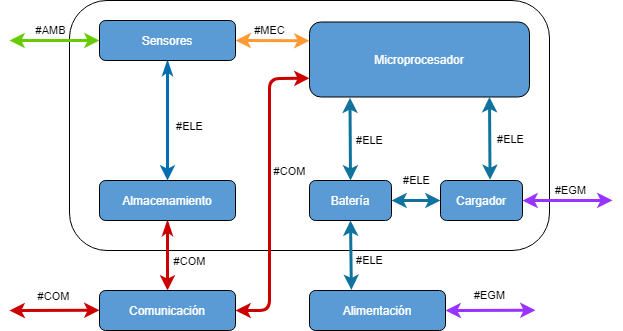
\includegraphics[width=0.8\linewidth]{ImagenesFactibilidad/EsquemaModular}
	\label{fig:esquema_modular}
	\caption{Diagrama modular del sistema.}
\end{figure}

\Subsubsection{Propuesta de sensores}

Para las distintas mediciones se tuvieron en cuenta diversas tecnologías que existen, poniendo en la balanza parámetros que definen su performance, tales como la linealidad de su salida, el costo, el rango de operación, la precisión, el tipo de salida, aplicación, entre otras tantas variables.

\Subsubsubsection{Temperatura}
En el caso de la medición de temperatura, se valoraron diversas tecnologías que existen, siendo por ejemplo la RTD cuyo funcionamiento se basa en el cambio de la resistencia en función de la temperatura bajo al ecuación $R(T)=R_0 + \alpha \cdot \Delta T$. También se consideró la tecnología TC, cuyo funcionamiento se basa en el \textit{efecto seebek}. Finalmente, el uso de un IC, el cual se basa en propiedades de dispositivos semiconductores extrínsecos.

\begin{table}[H]
\centering
\begin{tabular}{|c|c|c|c|c|}
\hline
\textbf{\begin{tabular}[c]{@{}c@{}}Aspectos\\ comparativos\end{tabular}} & \textbf{\href{https://www.thermocoupleinfo.com/type-k-thermocouple.htm}{TC-K}}                                                                             & \textbf{\href{http://www.datasheet.es/PDF/900325/Pt100-pdf.html}{PT-100}}                                                                                                              & \textbf{\href{https://datasheets.maximintegrated.com/en/ds/DS18B20.pdf}{Ds18b20}}                                                 & \textbf{\href{https://www.sparkfun.com/datasheets/Sensors/Temperature/DHT22.pdf}{DHT-22}}  \\ \hline
\textbf{Costo [ARS]}                                                           & 700	& 780	& 200	& 740	\\ \hline
\textbf{Tipo de salida}                                                  & Analógico                                                                                 & Analógico                                                                                                                    & Digital                                                          & Digital          \\ \hline

\textbf{\begin{tabular}[c]{@{}c@{}}Rango de\\ operación [°C]\end{tabular}}                                              & -40 $\sim$ 1200                                                                        & -50 $\sim$ 200  & -10 $\sim$ 85 & -40 $\sim$ 80 \\ \hline
\textbf{\begin{tabular}[c]{@{}c@{}}Interfaz de\\ conexionado\end{tabular}}                                                      & \begin{tabular}[c]{@{}c@{}}Se debe\\ proporcionar\\ un circuito\\ amplificador\end{tabular} & \begin{tabular}[c]{@{}c@{}}Se debe \\ proporcionar\\  un circuito\\  convertidor\\  de resistencia\\  a tensión\end{tabular} & -                                                                & -                \\ \hline
\textbf{Presición [°C]}                                                       & $\pm$ 1.5	& $\pm$ 0.1	& $\pm$ 0.5	& $\pm$ 0.5	\\ \hline

\textbf{Estabilidad}                                                     & Tienden a envejecer                                                                       & -                                                                                                                            & -                                                                & -                \\ \hline
\textbf{Autocalentamiento}                                               & -                                                                                         & \begin{tabular}[c]{@{}c@{}}Depende de\\  la corriente\\  de medición.\end{tabular}                                           & Bajo                                                             & Bajo             \\ \hline
\textbf{Imagen}                &  \includeintable{.1}{ImagenesFactibilidad/TC}                                                                                          &  \includeintable{.1}{ImagenesFactibilidad/PT100}                                                                                                                    & \includeintable{.1}{ImagenesFactibilidad/IC1}  &  \includeintable{.1}{ImagenesFactibilidad/DHT-22}                 \\ \hline
\end{tabular}
\caption{Comparación entre sensores de temperatura.}
\end{table}

\Subsubsubsection{Humedad}
Existen varias maneras de medir la magnitud física de la humedad, dentro de estas la mas común se basa en utilizar la dependencia que existe entre la humedad y la capacidad. Es por esto que se utilizan capacitores con un dieléctrico, el cual cambia constante con la humedad. Además existen sensores que se aprovechan de como cambia la resistencia en función de la temperatura, pero estas tecnologías son menos frecuentes.

\begin{table}[H]
\centering
\begin{tabular}{|c|c|c|c|c|}
\hline
\textbf{\begin{tabular}[c]{@{}c@{}}Aspectos\\ comparativos\end{tabular}} & \textbf{\href{https://www.mouser.com/datasheet/2/758/DHT11-Technical-Data-Sheet-Translated-Version-1143054.pdf}{DHT-11}}   & \textbf{\href{http://codigoelectronica.com/blog/am2301-datasheet}{AM-2301}}  & \textbf{\href{https://www.sparkfun.com/datasheets/Sensors/Temperature/DHT22.pdf}{DHT-22}}   & \textbf{\href{https://datasheetspdf.com/pdf/1298922/AOSONG/AM1001/1}{AM-1001}}  \\ \hline
\textbf{Costo [ARS]}                                                           & 200           & 1050 & 740 & 840	\\ \hline
\textbf{\begin{tabular}[c]{@{}c@{}}Rango de\\ operación [\%RH]\end{tabular}}                                              & 20 $\sim$ 90 & 0 $\sim$ 100 & 0 $\sim$ 100 & 20 $\sim$ 90 \\ \hline
\textbf{Presición [\%RH]}                                                       & $\pm$4	& $\pm$3	 & $\pm$2	& $\pm$5	\\ \hline
\textbf{Tipo de salida}                                                  & Digital           & Digital           & Digital           & Analógica         \\ \hline
\textbf{Imagen}                                                          & \includeintable{.1}{ImagenesFactibilidad/DHT-11}                 & \includeintable{.1}{ImagenesFactibilidad/AM-2301}                 & \includeintable{.1}{ImagenesFactibilidad/DHT-22}                 & \includeintable{.1}{ImagenesFactibilidad/AM-1001} \\ \hline
\end{tabular}
\caption{Comparación de sensores de humedad.}
\end{table}

\Subsubsubsection{Luminosidad}
En la medición del nivel de luminosidad se puede optar por diversos caminos. Existen sensores como el BH-1750 y OPT-100 que su funcionamiento se basa en un fotodiodo que conduce cierta corriente a partir de la luz que le impacta. Otros sensores, tales como el TEMT-600, emplean un fototransistor, cuya base se encuentra expuesta. En función de la intensidad lumínica en dicha zona, circulará cierta corriente por el colector. Finalmente existen fotoresistores, los cuales, tal como su nombre indica, cambian la resistencia en función del nivel de luz.
\begin{table}[H]
\centering
\begin{tabular}{|c|c|c|c|c|}
\hline
\textbf{\begin{tabular}[c]{@{}c@{}}Aspectos\\ comparativos\end{tabular}}              & \textbf{\href{https://www.mouser.com/datasheet/2/348/bh1750fvi-e-186247.pdf}{BH-1750}}  & \textbf{\href{https://www.vishay.com/docs/81579/temt6000.pdf}{TEMT-6000}}	& \textbf{\href{https://www.ti.com/lit/ds/symlink/opt101.pdf}{OPT-101}}                                              & \textbf{\href{https://www.alldatasheet.es/view.jsp?Searchword=GL55}{GL55-LM393}} \\ \hline
\textbf{Costo [ARS]}	& 230 	& 340	& 330	& 190	\\ \hline
\textbf{\begin{tabular}[c]{@{}c@{}}Rango de \\ temperatura\\  de operación [°C]\end{tabular}} & -40 $\sim$ 85  & -40 $\sim$ 85 & 0 $\sim$ 70 & -30 $\sim$ 70 \\ \hline
\textbf{\begin{tabular}[c]{@{}c@{}}Potencia\\ disipada [mW]\end{tabular}}                                                            & 260 	& 100 	& \TBD 	& 75 	\\ \hline
\textbf{Tipo de salida}                                                               & I2C               & \begin{tabular}[c]{@{}c@{}}Analógica\\ (Corriente)\end{tabular}                 & \begin{tabular}[c]{@{}c@{}}Analógica\\ (Tensión)\end{tabular} &\begin{tabular}[c]{@{}c@{}}Analógica \\ Digital\end{tabular}  \\ \hline
\textbf{Aplicación}                                                                   & -                 & \begin{tabular}[c]{@{}c@{}}Necesita un\\amplificador\\ de corriente\end{tabular} & -                                                             & -                   \\ \hline
\begin{tabular}[c]{@{}c@{}}\textbf{Tensión de} \\ \textbf{alimentación [V]} \end{tabular}                                                      & 4.5 	& \textless \ 6 	& 2.7 $\sim$ 36.0 	& 3.3 $\sim$ 5.0 	\\ \hline
\textbf{\begin{tabular}[c]{@{}c@{}}Rango de\\ medición [nm]\end{tabular}}                                                            & 450 $\sim$ 650 & 400 $\sim$ 900 & 450 $\sim$ 1000 & 450 $\sim$ 750 \\ \hline
\textbf{Imagen}                                                                       & \includeintable{.1}{ImagenesFactibilidad/BH-1750} & \includeintable{.1}{ImagenesFactibilidad/TEMT-6000}                                                                               & \includeintable{.1}{ImagenesFactibilidad/OPT-101} & \includeintable{.1}{ImagenesFactibilidad/GL55-LM393}                   \\ \hline
\end{tabular}
\caption{Comparación de sensores de luminosidad.}
\end{table}

\Subsubsection{Elección de una solución}

\Subsubsubsection{Temperatura}

En cuanto al sensor de temperatura la primer opción a descartar es aquella que no cumple con el rango de temperaturas a medir, por lo que el Ds18b20 queda descartado a pesar de su bajo costo. Luego de las opciones que quedan todas son de un costo similar, sin embargo hay que tener en cuenta que para la termocupla se debe proporcionar una manera de medir la temperatura de referencia, la cual puede ser tanto una RTD como un IC. Es por esto que el costo de la termocupla aumentaría con creces. Tanto la TC como la RTD necesitan un circuito convertidor para poder medir directamente el valor de la temperatura con un micro controlador, mientras que los IC ofrecen directamente una salida digital. La mejor precisión de la medición se da con una RTD, seguido por los IC y finalmente la TC.

Una desventaja de la TC es que tiende a envejecer rápidamente. Si bien el estudio no dura mas de 3 meses, el producto podrá ser reutilizado, siendo dicho envejecimiento un problema. El autocalientamiento también es contraproductivo en la medición de temperatura debido a que este puede alterar la misma si no es tenido en cuenta. Las TC no cuentan con este inconveniente debido a su principio de funcionamiento, mientras que con las otras opciones si lo es. Con la RTD este efecto depende directamente con la corriente que se suministra para la medición, y con los IC es un aspecto que es considerado por los diseñadores de los mismos.

Por estas razones los candidatos a terminan siendo DHT-22 y la PT-100. Un punto favorable para la DHT-22 es que no necesita un circuito extra y el problema del autocalentamiento ya fue pensado. Adicionalmente esta unidad cuenta con una medición de humedad la cual podría usarse como sensor de humedad, ya siendo el principal o usado como complemento.

\Subsubsubsection{Humedad}
De las opciones vistas, como primer criterio, se busca que pueda medir el rango entero de la humedad relativa y que cuente con una precisión considerable. Dadas estas consideraciones, se descarta el DHT-11 y AM-1001. Es así que de los dos restantes, se opta por el DHT-22 debido a que por un menor costo se obtienen mejores prestaciones. Teniendo en cuenta esto se utilizará tanto para la medición de temperatura y humedad el DHT-22.

\Subsubsubsection{Luminosidad}
En la elección para esta medición, principalmente se deberá asegurar el funcionamiento en el rango de temperatura en el cual operará el dispositivo, por lo cual el OPT-101 queda descartado. Luego se tendrá en cuenta la potencia utilizada, el rango de medición de los sensores y el tipo de alimentación.

La comunicación puede ser analógica en corriente para el TEMT-6000, pero este necesitará un amplificador de corriente o un convertidor para esta corriente a un nivel medible. Existen también otros sensores que tienen una salida analógica de tensión como el GL55-LM393 con un rango entre 0 y VCC. Este también provee con una salida digital, pero esta funciona como un schmitt trigger. Finalmente el BJ-1750 cuanta con una salida digital con el protocolo de comunicación I2C.

Teniendo en cuenta esto se opta por utilizar el sensor \TBD.

\Subsection{Propuesta de almacenamiento}

\begin{table}[H]
\centering
\begin{tabular}{|c|c|c|c|}
\hline
\textbf{\begin{tabular}[c]{@{}c@{}}Aspectos\\ comparativos\end{tabular}}         & \textbf{\href{https://www.kingston.com/datasheets/sdcg3_es.pdf}{SDCG3}} & \textbf{\href{https://www.kingston.com/datasheets/mlpmr2_es.pdf}{SDCE}} & \textbf{\href{https://ar.mouser.com/datasheet/2/669/SanDisk_02052018_SDSDAF3_SDSDQAF3-1285144.pdf}{SDSDQAF3-XI}} \\ \hline
\textbf{Costo [ARS]}                                                             & 2100 $\sim$ 3900                                                        & 7900 $\sim$ 15000                                                       & 7600 $\sim$ 17000                                                                                                 \\ \hline
\textbf{\begin{tabular}[c]{@{}c@{}}Temperatura de\\ operación [°C]\end{tabular}} & -25 $\sim$ 85                                                           & -25 $\sim$ 85                                                           & -40 $\sim$ 85                                                                                                    \\ \hline
\textbf{Almacenamiento [GB]}                                                     & 64 $\sim$ 512                                                           & 64 $\sim$ 256                                                           & 8 $\sim$ 128                                                                                                     \\ \hline
\textbf{\begin{tabular}[c]{@{}c@{}}Velocidad\\ R/W [MB/s]\end{tabular}}          & 170 / 90                                                                & 285 / 165                                                               & 50 / 80                                                                                                          \\ \hline
\textbf{Alimentación [V]}                                                        & 3.3                                                                     & 3.3                                                                     & 2.7 $\sim$ 3.6                                                                                                   \\ \hline
\textbf{Imagen}                                                                  & \includeintable{.1}{ImagenesFactibilidad/SDCG3}                         & \includeintable{.1}{ImagenesFactibilidad/SDCE}                          & \includeintable{.1}{ImagenesFactibilidad/SDSDQAF3}                                                               \\ \hline
\end{tabular}
\caption{Comparación entre memorias SD.}
\end{table}

\Subsection{Propuesta de comunicación}

\Subsection{Propuesta de microprocesador}

\begin{table}[H]
\centering
\begin{tabular}{|c|c|c|c|}
\hline
\textbf{\begin{tabular}[c]{@{}c@{}}Aspectos\\ comparativos\end{tabular}}         & \textbf{\href{https://datasheets.raspberrypi.org/rpi4/raspberry-pi-4-product-brief.pdf}{R-Pi 4}} & \textbf{\href{https://www.raspberrypi.org/products/raspberry-pi-zero/}{R-Pi Zero W}}            & \textbf{\begin{tabular}[c]{@{}c@{}}\href{https://datasheets.raspberrypi.org/cm4/cm4-product-brief.pdf}{R-Pi Compute}\\ \href{https://datasheets.raspberrypi.org/cm4/cm4-product-brief.pdf}{Module 4}\end{tabular}} \\ \hline
\textbf{Costo [ARS]}                                                                   & 10400 $\sim$ 17000                                                                               & 6000 $\sim$ 7500                                                                                & 12440 $\sim$ 14310                                                                                                                                                                                                 \\ \hline
\textbf{\begin{tabular}[c]{@{}c@{}}Temperatura de\\ operación [°C]\end{tabular}} & 0 $\sim$ 50                                                                                      & -                                                                                               & -20 $\sim$ 85                                                                                                                                                                                                      \\ \hline
\textbf{Memoria [GB]}                                                            & 1 $\sim$ 8                                                                                       & 512                                                                                             & 1 $\sim$ 8                                                                                                                                                                                                         \\ \hline
\textbf{Conexiones}                                                              & \begin{tabular}[c]{@{}c@{}}Wireless LAN,\\ Bluetooth,\\ Ethernet, USB\end{tabular}               & \begin{tabular}[c]{@{}c@{}}Wireless LAN,\\ Bluetooth (BLE),\\ Micro USB, mini HDMI\end{tabular} & \begin{tabular}[c]{@{}c@{}}Wireless LAN,\\ Bluetooth,\\ Ethernet, USB,\\ antena externa\end{tabular}                                                                                                               \\ \hline
\textbf{Sonido y video}                                                          & \begin{tabular}[c]{@{}c@{}}Micro HDMI,\\ MIPI DSI y CSI\end{tabular}                             & \begin{tabular}[c]{@{}c@{}}Mini HDMI, HDMI,\\ CSI, PAL/NTSC pads\end{tabular}                   & \begin{tabular}[c]{@{}c@{}}HDMI, MIPI DSI\\ y CSI, SDIO\end{tabular}                                                                                                                                               \\ \hline
\textbf{Soporte SD}                                                              & \begin{tabular}[c]{@{}c@{}}Almacenamiento y\\ carga de SO\end{tabular}                           & Micro SD                                                                                        & \begin{tabular}[c]{@{}c@{}}Entrada SD para tarjeta\\ o eMMC externo\end{tabular}                                                                                                                                   \\ \hline
\textbf{Dimensiones [mm]}                                                        & 85.6 x 56.5                                                                                      & 65 x 30                                                                                         & 40 x 55 x 1.2                                                                                                                                                                                                      \\ \hline
\textbf{Alimentación}                                                            & 5 V (3 A)                                                                                        & 5 (1.2 A)                                                                                       & 5 V (1.4 A)                                                                                                                                                                                                        \\ \hline
\textbf{Imagen}                                                                  & \includeintable{.1}{ImagenesFactibilidad/RPI4}                                                   & \includeintable{.1}{ImagenesFactibilidad/RPIZero}                                               & \includeintable{.1}{ImagenesFactibilidad/RPICM}                                                                                                                                                                    \\ \hline
\end{tabular}
\caption{Comparación entre palcas Raspberry Pi.}
\end{table}

\Subsection{Propuesta de batería}

\begin{table}[]
\centering
\begin{tabular}{|c|c|c|c|c|}
\hline
\textbf{\begin{tabular}[c]{@{}c@{}}Aspectos\\ comparativos\end{tabular}}                          & \textbf{\href{https://www.kijo-battery.com/products/jdg-series-agm-gel-deep-cycle-battery.html}{Kijo Serie JDG}} & \textbf{\href{https://www.kijo-battery.com/products/jlg-series-pure-gel-deep-cycle-battery.html}{Kijo Serie JLG}} & \textbf{\href{http://www.fenk.com.ar/wp-content/uploads/2020/01/JS12-20-1.pdf}{Fenk JS12-20}} & \textbf{\href{http://www.fenk.com.ar/productos/energias-renovables/baterias-solares/}{Fenk Serie JM12}} \\ \hline
\textbf{Costo [ARS]}                                                                              & 30500 $\sim$ X                                                                                                   & X $\sim$ X                                                                                                        & 6365 $\sim$ 8744                                                                              & 20332 $\sim$ 76110                                                                                      \\ \hline
\textbf{\begin{tabular}[c]{@{}c@{}}Temperatura de\\ operación [°C]\end{tabular}}                  & -20 $\sim$ 50                                                                                                    & -20 $\sim$ 50                                                                                                     & -20 $\sim$ 50                                                                                 & -20 $\sim$ 50                                                                                           \\ \hline
\textbf{\begin{tabular}[c]{@{}c@{}}Tensión\\ nominal [V]\end{tabular}}                            & 12                                                                                                               & 12                                                                                                                & 12                                                                                            & 12                                                                                                      \\ \hline
\textbf{Capacidad [Ah]}                                                                           & 33 $\sim$ 250                                                                                                    & 100 $\sim$ 200                                                                                                    & 13.2 $\sim$ 20.0                                                                              & 32.7 $\sim$ 200.0                                                                                       \\ \hline
\textbf{\begin{tabular}[c]{@{}c@{}}Dimensiones\\ (máximas) [mm]\end{tabular}}                     & 52 x 268 x 220                                                                                                   & 499 x 259 x 219                                                                                                   & 181 x 77 x 167                                                                                & 522 x 240 x 219                                                                                         \\ \hline
\textbf{Peso [kg]}                                                                                & 10 $\sim$ 61                                                                                                     & 30 $\sim$ 74                                                                                                      & 5.45                                                                                          & 15.5 $\sim$ 57.0                                                                                        \\ \hline
\textbf{\begin{tabular}[c]{@{}c@{}}Porcentaje de\\ autodescarga\\ (mensual a 25 °C)\end{tabular}} & 3\%                                                                                                              & 3\%                                                                                                               & 3\%                                                                                           & 3\%                                                                                                     \\ \hline
\textbf{Imagen}                                                                                   & \includeintable{.1}{ImagenesFactibilidad/Kijo-JDG}                                                               & \includeintable{.1}{ImagenesFactibilidad/Kijo-JLG}                                                                & \includeintable{.1}{ImagenesFactibilidad/Fenk-JS12-20}                                        & \includeintable{.1}{ImagenesFactibilidad/Fenk-JM12}                                                     \\ \hline
\end{tabular}
\caption{Comparación entre baterías gel de carga profunda.}
\end{table}

\Subsection{Propuesta de cargador}

\Subsection{Propuesta de alimentación}

\begin{table}[H]
\centering
\begin{tabular}{|c|c|c|}
\hline
\textbf{\begin{tabular}[c]{@{}c@{}}Aspectos\\ comparativos\end{tabular}}                   & \textbf{DSP-20P} & \textbf{DSP-30M} \\ \hline
\textbf{\begin{tabular}[c]{@{}c@{}}Temperatura de\\ operación [°C]\end{tabular}}           & -45 $\sim$ 85    & -45 $\sim$ 85    \\ \hline
\textbf{\begin{tabular}[c]{@{}c@{}}Potencia\\ máxima [W]\end{tabular}}                     & 20 $\pm$ 3\%     & 30 $\pm$ 3\%     \\ \hline
\textbf{\begin{tabular}[c]{@{}c@{}}Tensión a\\ potencia\\ máxima [V]\end{tabular}}         & 17.6             & 18               \\ \hline
\textbf{\begin{tabular}[c]{@{}c@{}}Corriente\\ a potencia\\ máxima [A]\end{tabular}}       & 1.14             & 1.67             \\ \hline
\textbf{\begin{tabular}[c]{@{}c@{}}Tensión a\\ circuito abierto\\ máxima [V]\end{tabular}} & 22.0             & 21.5             \\ \hline
\textbf{\begin{tabular}[c]{@{}c@{}}Corriente a\\ corto circuito\\ máxima [A]\end{tabular}} & 1.39             & 1.86             \\ \hline
\end{tabular}
\caption{Comparación entre paneles solares.}
\end{table}


\Subsubsection{DFMEA}

\Subsection{Factibilidad de tiempos}

\Subsubsection{Planificación}
(PERT y simulación de Montecarlo)

\Subsubsection{Programación}
(Gantt)

%\Subsection{Factibilidad económica}
%(Mercado, costos, ciclo de vida, VAN, TIR)

\Subsection{Factibilidad legal y responsabilidad civil}
(regulaciones y licencias)

\end{document}